\documentclass{article}

% if you need to pass options to natbib, use, e.g.:
% \PassOptionsToPackage{numbers, compress}{natbib}
% before loading nips_2017
%
% to avoid loading the natbib package, add option nonatbib:
% \usepackage[nonatbib]{nips_2017}

\usepackage[final]{nips_2017}


\usepackage[utf8]{inputenc} % allow utf-8 input
\usepackage[T1]{fontenc}    % use 8-bit T1 fonts
\usepackage{hyperref}       % hyperlinks
\usepackage{url}            % simple URL typesetting
\usepackage{booktabs}       % professional-quality tables
\usepackage{amsfonts}       % blackboard math symbols
\usepackage{nicefrac}       % compact symbols for 1/2, etc.
\usepackage{microtype}      % microtypography
\usepackage{booktabs}
\usepackage{natbib}
\usepackage{graphicx}
\usepackage{array}
\usepackage{caption}
\usepackage{multirow}
\usepackage{subcaption}

\newcommand\Tstrut{\rule{0pt}{2.1ex}}       % "top" strut

% Choose a title for your submission
\title{NLU: Story Cloze Task - Report}


%\author{Student 1 \\ pblatter@student.ethz.ch \qquad Student 2 \qquad Student 3}
\author{
  \textbf{Blatter Philippe}\\
  ETH Zürich \\
  \texttt{pblatter@ethz.ch}
  \and
  \textbf{Brunner Lucas} \\
  ETH Zürich \\
  \texttt{brunnelu@ethz.ch}
  \and
  \textbf{Küchler Nicolas}\\
  ETH Zürich \\
  \texttt{kunicola@ethz.ch}
}

\begin{document}
% \nipsfinalcopy is no longer used

\maketitle

\section{Introduction}

The Story Cloze Task \cite{SCT} requires a system to choose the correct \textit{ending} to a four-sentence story (\textit{context}).
The task poses two major challenges:

\begin{enumerate}
    \item \emph{Story Understanding}: The data contains a rich set of causal and temporal common sense relations which are hard for an algorithm.
    In order to come close to human performance, a powerful model which is able to understand the story is almost certainly required.
    \item \emph{Training Dataset}: The ROC corpus does not contain negative samples (i.e. stories with wrong endings). At first, this does not sound problematic but it turns out that generating a training set which is representative for the validation- and test set is not straightforward.
\end{enumerate}

\section{Methodology}

After experimenting with a baseline from the area of stance detection based on a model used in the first fake news challenge \cite{FNC}, we realized that the Story Cloze Task requires a more powerful and sophisticated model.
We decided to use the language representation model BERT, pre-trained on multiple large corpora including Wikipedia.
The model is fine-tuned for the Story Cloze Task with an additional output layer to calculate how well an ending matches the given context.
In order to discriminate between the two context-ending pairs, the probabilities are compared. The same or a similar approach has proven to produce state-of-the-art results on comparable tasks such as the GLUE benchmark or the SWAG dataset \cite{BERT}.

The focus of this work lies on generating a useful training set from the provided stories.
A naïve approach would be to sample a false ending uniformly at random from all other story endings.
However, this poses the problem that the resulting training set is quite different compared to the validation- and test set (e.g. the actor of the story changes, the ending is about an unrelated topic). We propose a set of simple heuristics and ideas to construct a better dataset that adapts over time and show that it improves performance.

\section{Model}\label{sec:model}

\subsection{BERT}\label{ssec:bert}
BERT stands for Bidirectional Encoder Representations from Transformers
and is a deep neural network architecture designed to pre-train deep bidirectional representations from unlabeled text \cite{BERT}. 
In this work, we use the uncased BERT-Base model with a sequence length of 128.
The model consists of 12-layers and has 110M parameters in total.

\subsection{Name replacement}\label{ssec:namerepl}
Most stories have an actor which is recurring throughout the story.
Consequently, sampling a random false ending can easily be detected by a powerful model simply based on the sudden change of actor in the last sentence.
Therefore, we came up with a simple heuristic that extracts the actor of both the context and the false ending. Afterwards, the ending's actor is replaced by the context's actor.

% [NKU] Proposal Instead of Next paragraph:
In the beginning, we used named entity recognition of the Stanford CoreNLP software \cite{finkel-etal-2005-incorporating} to extract the actors from the story.
However, we abandoned this approach quickly because the actors in the training-, validation- and test set are almost always called by their first name.
As a result, the simple approach of first tokenizing the sentences and then using a first name dataset \cite{Name_database} to check for actors resulted in more convincing results.

\subsection{Embedding}\label{ssec:embedding}

Using random false endings usually creates stories in which context and ending are unrelated. In order to circumvent this issue, we trained embeddings of the story titles using Doc2Vec\cite{Doc2Vec}. We generated negative samples by combining context and ending of two stories whose titles are close to each other in the embedding space. This approach is based on the presumption that such samples are harder to classify and hence increase the discriminative power of the model.

For comparison purposes, we trained a second embedding on the entire stories.
In both embeddings all names are replaced with an \textit{unknown} tag because this is already handled by the name replacement described in \ref{ssec:namerepl}.

\subsection{Adaptive Data Set}\label{ssec:adaptive_dataset}
The idea of the adaptive dataset is that the correct context-ending pairs remain the same but the incorrect ones are changed in every epoch while maintaining a balanced dataset.
To be more precise, the dataset for the first epoch is the dataset based on story title similarity as described in section \ref{ssec:embedding}.
After each epoch, every story context $c_{i}$ is evaluated against a set of false endings $D_{i}$.
The negative samples for the next epoch are then constructed by taking the false endings which BERT considers to be the most likely.
The motivation behind this is that these are the challenging samples from which BERT can learn the most in the next epoch.

\begin{equation}
(c_i, e) = {argmax_e} {P(e|c_i)} \qquad \forall i =\{1, \cdots , n\} \qquad  e \in D_i
\end{equation}

Ideally, we would like to check all possible context ending pairs (i.e. cross-product: $|D_i| = n-1$) to find negative samples which the model classifies as plausible.
However, this would result in a dataset in the order of $\mathcal{O}(n^2)$ which is not feasible for $n=88'161$ training stories because the process of predicting would take too long.
As an approximation, only the endings of the top 20 most similar stories are checked instead of all ($n-1$) false endings. 
The similarity between stories is calculated based on the story title as described in section \ref{ssec:embedding} . $D_i = D_{top 20 title}$

The underlying assumption of the whole adaptive dataset approach is that every story context has only one plausible ending in the dataset.
Even though this is probably not always satisfied, the experimental results suggest that the benefit of finding challenging endings outweighs the introduced error in the dataset.

\subsection{Fake News Challenge UCL Model}\label{ssec:fnc-stance}
A completely different approach used as a baseline was to compare the stances of the context and the endings. As the context and the inherent correct ending are closely related, their stances should be similar too. 
In order to see whether the stance of the context matches the stance of a given ending, we used a model from the first fake news challenge \cite{FNC}.
The task of this challenge was to decide the stance of a headline to the body of a news article. In a retrospective analysis of this challenge a model from UCL performed almost as good as the best models but with a much simpler approach 
\cite{A_Retrospective_Analysis_of_the_Fake_News_Challenge}. The model only consists of one hidden layer of size 100 and an input layer consisting of the term frequency vectors of the context and the ending and the cosine similarity of the tf-idf vectors from both. To counter overfitting l2 regularization and dropout layers are used. The size of those vectors depends on the vocabulary size. As stop words do not give much more information in this setting, they are removed from the vocabulary. Because the performance of their code was not that well we rewrote it and further optimized it.


\section{Training}

In the BERT training, each sample is a triple of (context, ending, label) where label $\in \{0,1\}$ depending on whether context and ending are forming a valid five sentence story.
After loading the provided pre-trained weights, the BERT model is fine-tuned for the Story Cloze Task with 3 epochs and a batch size of 32. During the fine-tuning, the binary cross-entropy loss function is optimized using the Adam optimizer with a learning rate of 2e-5. The process of pre-training BERT along with the hyperparameters are described in \cite{BERT}.

In the training of the Fake News Challenge UCL Model, most parameters stay the same as in the original model \cite{UCL_model}. We use the Adam optimizer with a learning rate of 0.01 to optimize the binary cross-entropy loss. The model is trained for 50 epochs and a vocabulary size of 10000 is used. The optimal vocabulary size was found through a grid search.


\section{Experiments}
\subsection{Using ROC Training Set for Training}

\emph{Adaptive Dataset with Name Replacement} is the complete approach.
BERT is fine-tuned on the training set generated by applying the name replacement and the adaptive dataset approach (see sections \ref{ssec:namerepl}, \ref{ssec:embedding} and \ref{ssec:adaptive_dataset}).
In order to gain a better understanding of the effects of the individual parts of the training set generation, we present an ablation study:

\begin{enumerate}
    \item \emph{Ablation Study 1: Without Name Replacement} serves as a baseline. The false samples are constructed by the naïve approach of sampling a random false ending form the other stories in the training set.
    \item \emph{Ablation Study 2: With Name Replacement} uses randomly sampled false endings and applies the name replacement according to section \ref{ssec:namerepl}.
    \item \emph{Ablation Study 3: Title Embedding} makes use of the story title embeddings to add  false endings as described in section \ref{ssec:embedding}.
    \item \emph{Ablation Study 4: Story Embedding} uses the story embeddings to construct false samples as shown in section \ref{ssec:embedding}.
\end{enumerate}

\emph{Stance Detection} is the baseline using the approach discussed in section \ref{ssec:fnc-stance}.

\subsection{Using ROC Training Set and Validation Set for Training}

Previous work \cite{DBLP:journals/corr/abs-1803-05547} suggests that using the validation set for training is very beneficial to the performance on the test set.
In order to verify this observation we perform two experiments: 
\begin{enumerate}
\item \emph{Training: Valid Only} fine-tunes BERT only on the validation set for 3 epochs
\item \emph{Training: Train + Valid} fine-tunes BERT on the training set as described above and runs one additional epoch of fine-tuning on the validation set
\end{enumerate}

\begin{table}[h]
\centering
\vspace{-1mm}
\begin{tabular}{clcc}  
    \hline
     & Experiment    & Validation Accuracy & Test Accuracy \Tstrut \\
    \hline
    \parbox[t]{1mm}{\multirow{7}{*}{\rotatebox[origin=c]{90}{BERT}}} 
    & Adaptive Dataset with Name Replacement              & 0.745         & \textbf{0.742} \Tstrut  \\
    & Training: Valid Only                                & 0.988         & 0.872                   \\
    & Training: Train + Valid                             & 0.966         & \textbf{0.877}          \\
    & Ablation Study 1: Without Name Replacement          & 0.616         & 0.618                   \\
    & Ablation Study 2: With Name Replacement             & 0.690         & 0.680                   \\
    & Ablation Study 3: Title Embedding                   & 0.722         & 0.726                   \\
    & Ablation Study 4: Story Embedding                   & 0.727         & 0.700                   \\
    \hline
    \parbox[t]{2mm}{\multirow{2}{*}{\rotatebox[origin=c]{90}{VAR}}} 
    & Stance Detection                                    & 0.573         & 0.565      \Tstrut      \\
    & LSDSem'17 Winner: msap                              & -             & 0.752                   \\
    \hline
\end{tabular}
\vspace{1mm}
\caption{Accuracy scores achieved by the different experiments on the ROC validation and test sets. The result from the LSDMSem'17 Winner are from \cite{mostafazadeh-etal-2017-lsdsem} and is listed as a reference.}
\label{table_acuracy}
\end{table}

\subsection{Results Analysis}

When only using the ROC training set for fine-tuning BERT, our approach with the adaptive dataset almost reaches state-of-the-art results from the LSDMSem'17 shared task \cite{mostafazadeh-etal-2017-lsdsem}.
However, one has to note that in particular the step of generating predictions for $20n$ samples is computationally expensive.

The ablation study further shows that each part of the dataset generation contributes to the performance on both validation and test set and hence strengthens the hypotheses from section \ref{sec:model}. The difference between using the embeddings from the title or from the complete story is small. Due to the better performance on the test set we used the title embeddings in the complete approach.

Figure \ref{distribution1} shows that the decision between two endings is often close when only using the training data. However, in almost two third of the close cases, our approach predicts the correct ending.

We confirm the results of previous work \cite{DBLP:journals/corr/abs-1803-05547} suggesting that training the model on the validation set boosts the performance significantly.
This result can have two interpretations. 
The first one is that the validation- and test set are very similar and BERT can easily exploit this without actually understanding the story. In this interpretation, the performance on the ETH test set could be problematic if it does not share the same characteristics due to a different creation process.
A second interpretation of the results is that even though the performance with the created training set from the ROC training set is pretty good, the dataset still does not represent difficult examples well enough and so BERT cannot learn to discriminate them.
In this interpretation, additionally using the validation set to also include these hard examples makes sense and should not pose a problem in the ETH test set.
The truth probably lies somewhere in between the two interpretations. We decided to use the combination of training on both training and validation set for our final prediction on the ETH test set. This is reasonable because the use of the additional training samples prevents completely overfitting some artefacts of the data generation process which could happen when only using the validation set for training.

\begin{figure}[h]
	\begin{subfigure}[b]{.45\linewidth}
		\centering
		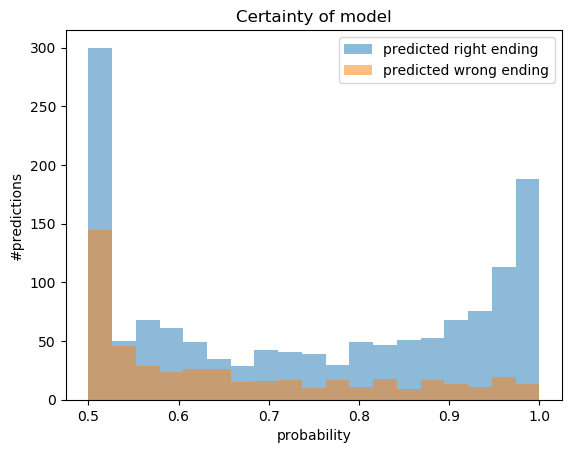
\includegraphics[width=\linewidth]{test_results_converted_t.png}
		\caption{Adaptive Dataset with Name Replacement}
	\end{subfigure}\hfill
	\begin{subfigure}[b]{.45\linewidth}
		\centering
		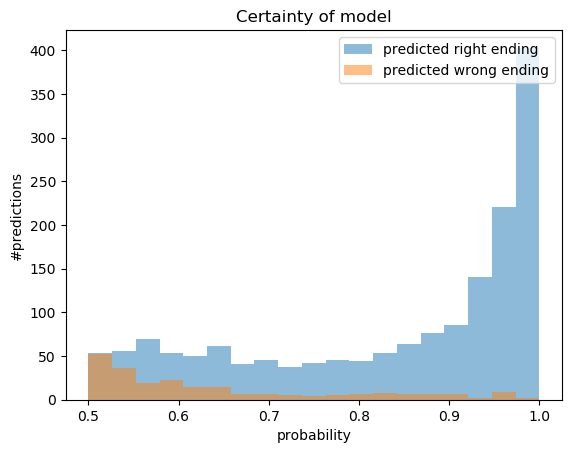
\includegraphics[width=\linewidth]{test_results_converted_tv.png}
		\caption{Training: Train + Valid}
	\end{subfigure}
	\caption{The normalized probabilities of the predictions on the test set. The normalization happens between the two context-ending pairs (e.g. for $(c,e1)$ and $(c,e2)$ BERT outputs 0.9 and 0.4 respectively, then $\frac{0.9}{0.9+0.4}$ is used in the histogram.)}\label{distribution1}
\end{figure}

\section{Conclusion}
We used the pre-trained uncased BERT-Base model to solve the Story Cloze Task with a specially constructed training dataset from the ROC Corpus training data.
Additionally, we analyzed the effect of including the validation data as training data.
Our experiments confirm that BERT is a good model for the Story Cloze Task if it is used in combination with an appropriate dataset.
However, the creation of such a good dataset from the ROC training corpus is not straightforward.

In future work, one could try the large BERT model which consistently performs better across many tasks \cite{BERT}. Another promising direction could be to feed both the positive and the negative sample to BERT at the same time and fine-tune the output layer to directly discriminate between the two choices. A similar approach was successfully used in the SWAG task \cite{BERT}.

%\nocite{*}
%\addcontentsline{chapter}{Bibliography}
\bibliographystyle{plain}
\bibliography{references}
\end{document}
